 \section{Durchführung}
Zur Bestimmung der Apperaturkonstanten $D$ und das Eigenträgheitsmoment $I_\text{D}$ der Drillachse wird eine Federwaage
eingehakt und um ein Winkel $\text{\phi}$ ausgelenkt. Es ist zu beachten, dass die Federwaage senkrecht zum Radius
gehalten wird, da sich das Kreuzprodukt vom Drehmoment aufhebt.
Mit der Formel aus (4) kann nun die Winkelrichtgröße berechnet werden.
Zur Bestimmung des Eigenträgheismoments wird ein masselosen Metallstab, an denen zwei Gewicht senkrecht zur Drehachse
befindet, angesteckt.
Das Trägheismoment verschiedener Objekte wird mithilfe der Formel (2) bestimmt.
Für eine Modelpuppe wird ebenfalls das Trägheitsmoment mithilfe der Formel (1) als auch (2) errechnet. Zur Vereinfachung wird
die Puppe aus verschiedenen Zylindern zusammengebaut (siehe Abbildung 3).
\begin{figure}
  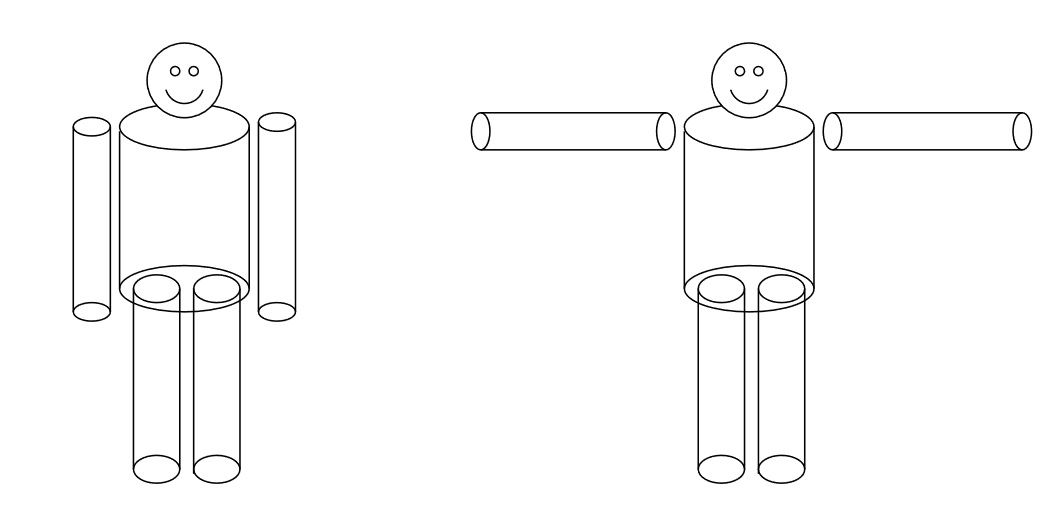
\includegraphics[width=\textwidth]{Bild3.jpg}
  \caption{Vereinfachte Darstellung der Modelpuppe[1]}
\end{figure}
